\section{Glasses, random media and two-level systems}\label{sec:16.7}

A superconducting resonator made on a film of thermally grown SiO$_2$ loses a fraction $3\times10^{-4}$ of its stored energy per radian at \SI{6}{GHz} and below \SI{100}{mK}, when it holds only a few photons~\cite[Table~I]{oconnell2008microwave}. At higher power or temperature the loss falls. The absorbers are groups of atoms in the glass that can sit in either of two configurations and tunnel between them, typically $10^{20}$ per eV and cm$^3$, with splittings that reach down to micro-electronvolts. At these energies a crystal has only its long acoustic phonons. The same systems absorb a dark photon of mass \SI{25}{\micro eV} as readily as a microwave photon of that energy, and a dark-matter particle that scatters in the glass can flip one of them. A glass is also the plainest example of a random medium. Its disorder raises two further questions: how its vibrations absorb a dark photon once momentum conservation no longer selects one optical phonon, and when a light particle that scatters coherently off a whole body can be treated in the Born approximation. The same tunneling systems release heat at millikelvin temperatures, and their kinetics are the subject of \cref{sec:16.8}.

\subsection{The standard tunneling model}\label{sec:16.7-stm}

Let $|\mathrm{L}\rangle$ and $|\mathrm{R}\rangle$ be the ground states of a group of atoms localized in the two wells of a double-well potential. In their span the Hamiltonian is \cref{eq:C.20-H} without the bath,
\begin{equation}
  H_{\mathrm{TLS}} = \tfrac12\Delta_{\mathrm{as}}\,\sigma_z - \tfrac12\Delta_0\,\sigma_x ,
  \qquad \Delta_{\mathrm{tl}} = \bigl(\Delta_{\mathrm{as}}^2 + \Delta_0^2\bigr)^{1/2} ,
  \label{eq:16.7-H}
\end{equation}
with the Pauli matrices of \cref{app:C.20} in the localized basis, the asymmetry $\Delta_{\mathrm{as}}$ between the two wells, the tunneling amplitude $\Delta_0$ and the splitting $\Delta_{\mathrm{tl}}$ of the eigenstates, the two-level splitting of \cref{sec:2.5}. The tunneling amplitude is exponentially small in the barrier, $\Delta_0 = \omega_{\mathrm{w}}\ee^{-\lambda_{\mathrm{tun}}}$, with $\omega_{\mathrm{w}} \sim$ the vibration energy in one well. For a particle of mass $M_{\mathrm{tun}}$ crossing a barrier of height $V_{\mathrm{b}}$ between wells a distance $d_{\mathrm{tun}}$ apart, the tunneling exponent is $\lambda_{\mathrm{tun}} = (d_{\mathrm{tun}}/2)(2M_{\mathrm{tun}}V_{\mathrm{b}})^{1/2}$~\cite[Sect.~II]{meissner2021acoustic}. In the eigenbasis the matrix $\sigma_z$, which measures in which well the atoms sit, becomes
\begin{equation}
  \sigma_z = \frac{\Delta_{\mathrm{as}}}{\Delta_{\mathrm{tl}}}\,\tau_z + \frac{\Delta_0}{\Delta_{\mathrm{tl}}}\,\tau_x ,
  \label{eq:16.7-rot}
\end{equation}
with $\tau_z$ and $\tau_x$ the Pauli matrices of the eigenstates and the sign of $\tau_x$ fixed by the phases of the eigenvectors. A perturbation that couples to the position of the atoms therefore drives transitions with the amplitude $\Delta_0/\Delta_{\mathrm{tl}}$: a system with $\Delta_0 \ll \Delta_{\mathrm{as}}$ has its eigenstates localized in the two wells, and the perturbation cannot move it from one to the other.

In a glass every system has its own $\Delta_{\mathrm{as}}$ and $\lambda_{\mathrm{tun}}$. The standard tunneling model of Phillips and of Anderson, Halperin and Varma takes both to be independent and uniformly distributed, with density $\bar P$ per unit asymmetry, unit exponent and unit volume~\cite[Eq.~(8)]{muller2019towards}. A system and its mirror image are the same system, so we count $\Delta_{\mathrm{as}} \ge 0$ only; this convention defines $\bar P$, and with both signs counted every rate below would carry a factor 2. Changing variables from $(\Delta_{\mathrm{as}}, \lambda_{\mathrm{tun}})$ to $(\Delta_{\mathrm{tl}}, \Delta_0)$, with $\dd\lambda_{\mathrm{tun}} = -\dd\Delta_0/\Delta_0$ and $\partial\Delta_{\mathrm{as}}/\partial\Delta_{\mathrm{tl}} = \Delta_{\mathrm{tl}}/\Delta_{\mathrm{as}}$ at fixed $\Delta_0$, gives
\begin{equation}
  P(\Delta_{\mathrm{tl}},\Delta_0) = \frac{\bar P\,\Delta_{\mathrm{tl}}}{\Delta_0\,(\Delta_{\mathrm{tl}}^2 - \Delta_0^2)^{1/2}} ,
  \qquad 0 < \Delta_0 \le \Delta_{\mathrm{tl}} ,
  \label{eq:16.7-P}
\end{equation}
the distribution of Ref.~\cite[Eq.~(12)]{meissner2021acoustic}. Its integral over $\Delta_0$ diverges logarithmically at small $\Delta_0$, and the number of systems per unit splitting depends on a lower cutoff of the tunneling amplitude that no experiment fixes. A transition probability, however, carries the weight $(\Delta_0/\Delta_{\mathrm{tl}})^2$ of \cref{eq:16.7-rot}, and
\begin{equation}
  \int_0^{\Delta_{\mathrm{tl}}}\dd\Delta_0\,P(\Delta_{\mathrm{tl}},\Delta_0)\,\frac{\Delta_0^2}{\Delta_{\mathrm{tl}}^2} = \bar P\int_0^1\frac{u\,\dd u}{(1 - u^2)^{1/2}} = \bar P ,
  \label{eq:16.7-norm}
\end{equation}
with $u = \Delta_0/\Delta_{\mathrm{tl}}$. The systems that dominate the count do not couple, and those that couple are counted by $\bar P$ alone, at every splitting. \Cref{fig:16-tls}(a) shows the two densities.

\begin{figure}[tbp]
  \centering
  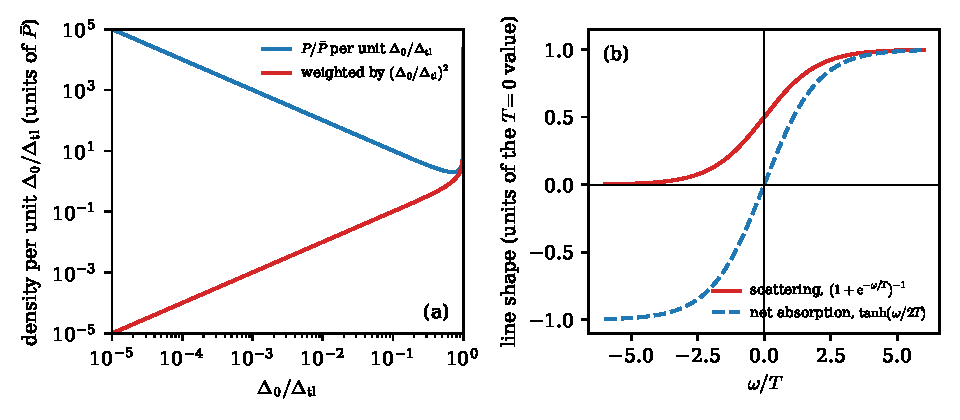
\includegraphics[width=\linewidth]{figures/ch16/fig16_7.pdf}
  \caption{The standard tunneling model. (a) Density of two-level systems per unit $u = \Delta_0/\Delta_{\mathrm{tl}}$ at fixed splitting, in units of $\bar P$: $1/[u(1 - u^2)^{1/2}]$ (blue), whose integral grows as $\ln(2/u_{\min})$ with the lower cutoff $u_{\min}$. Weighted by the squared transition amplitude $u^2$ (red), it integrates to one, \cref{eq:16.7-norm}; \SI{87}{\percent} of that comes from $u > 0.5$. (b) Line shapes of the ensemble at temperature $T$, in units of their $T = 0$ values. Red: the scattering structure factor $(1 + \ee^{-\omega/T})^{-1}$ of \cref{eq:16.7-S}, nonzero for $\omega < 0$ through the thermal population of the upper level; blue, dashed: the net absorption of a classical field, $\tanh(\omega/2T)$, \cref{eq:16.7-chires}.}
  \label{fig:16-tls}
\end{figure}

A strain field and an electric field both shift the energies of the two wells. The atoms move between configurations with different elastic and electric dipoles. To first order the asymmetry becomes $\Delta_{\mathrm{as}} + 2\gamma_{\mathrm{TLS}}u_{\mathrm{d}} + 2\vect{p}_{\mathrm{TLS}}\cdot\vect{E}$, with $u_{\mathrm{d}}$ the component of the strain tensor $u_{\alpha\beta}$ along the deformation of the defect, $\gamma_{\mathrm{TLS}}$ its deformation potential and $\vect{p}_{\mathrm{TLS}}$ half the difference of the electric dipoles of the two configurations~\cite[Eq.~(16)]{muller2019towards}. The perturbation is
\begin{equation}
  H_1 = \bigl(\gamma_{\mathrm{TLS}}u_{\mathrm{d}} + \vect{p}_{\mathrm{TLS}}\cdot\vect{E}\bigr)\,\sigma_z \equiv bF\,\sigma_z ,
  \label{eq:16.7-H1}
\end{equation}
where $F$ stands for the applied field ($u_{\mathrm{d}}$ or one component of $\vect{E}$) and $b$ for the coupling to it. By \cref{eq:16.7-rot} it has a transverse part, which drives transitions at $\omega = \Delta_{\mathrm{tl}}$, and a longitudinal part, which modulates the splitting.

The transverse part gives the resonant response. The power a field $F\cos\omega t$ deposits per unit volume is $\tfrac12\omega\chi''(\omega)F^2$, with $\chi''$ the absorptive part of the susceptibility of the coupled quantity $b\sigma_z$. For one system the golden rule of \cref{sec:2.1} gives an absorption rate from the lower level and an equal rate of stimulated emission from the upper one, and the populations of \cref{sec:2.5} differ by $p_0 - p_1 = \tanh(\Delta_{\mathrm{tl}}/2T)$. Hence $\chi''(\omega) = \pi b^2(\Delta_0/\Delta_{\mathrm{tl}})^2\tanh(\Delta_{\mathrm{tl}}/2T)\,\delta(\omega - \Delta_{\mathrm{tl}})$ for $\omega > 0$, where the delta function stands for the Lorentzian of \cref{eq:2.4-lorentz} with the width of the system, small against $\omega$ and $T$ in an insulating glass at millikelvin temperatures. Summing over the ensemble with \cref{eq:16.7-P,eq:16.7-norm},
\begin{equation}
  \chi''_{\mathrm{res}}(\omega) = \pi\bar P\,\langle b^2\rangle\,\tanh\frac{\omega}{2T} ,
  \label{eq:16.7-chires}
\end{equation}
independent of $\omega$, with $\langle b^2\rangle$ averaged over the orientations of the systems. Its two physical cases are the dielectric loss and the acoustic loss. For the electric field the orientation average is $\langle(\vect{p}_{\mathrm{TLS}}\cdot\hat{\vect{E}})^2\rangle = p_{\mathrm{TLS}}^2/3$, and in Heaviside--Lorentz units the polarization is $\chi\vect{E}$, so the imaginary part of the permittivity is $\chi''$ itself. Against the real part $\varepsilon_r$ of the glass, the loss tangent is
\begin{equation}
  \tan\delta(\omega,T) = \frac{\varepsilon_2}{\varepsilon_r} = \tan\delta_0\,\tanh\frac{\omega}{2T} , \qquad
  \tan\delta_0 = \frac{\pi\bar P\,p_{\mathrm{TLS}}^2}{3\varepsilon_r} ,
  \label{eq:16.7-tand}
\end{equation}
the low-power loss tangent $\tan\delta_0$ at $T \to 0$. For a sound wave of polarization $j$, longitudinal or transverse, the coupling is the deformation potential $\gamma_j$ and the elastic modulus $\rho_Tc_j^2$ takes the place of $\varepsilon_r$, so the internal friction is $Q^{-1} = \pi C_j\tanh(\omega/2T)$, with the tunneling strength $C_j = \bar P\gamma_j^2/\rho_Tc_j^2$~\cite[Eqs.~(5), (6)]{buchenau2020sound}. Both are the response of the standard tunneling model to a classical field~\cite[Eqs.~(4), (12), (13), (15)]{meissner2021acoustic}. In vitreous silica $C = 2.6\times10^{-4}$ on average over the two polarizations~\cite[Table~I]{buchenau2020sound}, and Golding, Graebner and Schutz find $C_{\mathrm{l}} = 1.9\times10^{-4}$ and $C_{\mathrm{t}} = 2.0\times10^{-4}$ at \SI{500}{MHz}, as quoted by Buchenau et al.~\cite[Sect.~III]{buchenau2020sound}.

The longitudinal part of \cref{eq:16.7-H1}, $bF(\Delta_{\mathrm{as}}/\Delta_{\mathrm{tl}})\tau_z$, shifts the splitting by $2bF\Delta_{\mathrm{as}}/\Delta_{\mathrm{tl}}$. In equilibrium the population difference would follow the shifted splitting at once; in fact it relaxes toward it at the rate $\varGamma_1 = 1/\tau_1$ of the system. The static susceptibility of the coupled quantity is $2b^2(\Delta_{\mathrm{as}}/\Delta_{\mathrm{tl}})^2\,\partial_{\Delta_{\mathrm{tl}}}\tanh(\Delta_{\mathrm{tl}}/2T)$, and a population that relaxes with one time constant turns it into the Debye form $\chi_{\mathrm{rel}}(\omega) = \chi_{\mathrm{rel}}(0)/(1 - \ii\omega\tau_1)$, whose absorptive part is $\chi_{\mathrm{rel}}(0)\,\omega\tau_1/(1 + \omega^2\tau_1^2)$~\cite[Eq.~(6)]{meissner2021acoustic}. In an insulating glass $\varGamma_1$ is set by the emission and absorption of one thermal phonon,
\begin{equation}
  \varGamma_1 = K_{\mathrm{ph}}\,\Delta_{\mathrm{tl}}^3\Bigl(\frac{\Delta_0}{\Delta_{\mathrm{tl}}}\Bigr)^2\coth\frac{\Delta_{\mathrm{tl}}}{2T} , \qquad
  K_{\mathrm{ph}} = \frac{1}{2\pi\rho_T}\Bigl(\frac{\gamma_{\mathrm{l}}^2}{c_{\mathrm{LA}}^5} + \frac{2\gamma_{\mathrm{t}}^2}{c_{\mathrm{TA}}^5}\Bigr) ,
  \label{eq:16.7-tau1}
\end{equation}
which \cref{sec:16.8} derives~\cite[Eq.~(7)]{meissner2021acoustic}. Summed over the ensemble and divided by the resonant value at $T = 0$, the full loss is
\begin{equation}
  \frac{\tan\delta}{\tan\delta_0} = \tanh\frac{\omega}{2T} + \frac{2}{\pi}\int_0^\infty\frac{\dd\Delta_{\mathrm{tl}}}{2T}\,\mathrm{sech}^2\frac{\Delta_{\mathrm{tl}}}{2T}\int_0^1\dd u\,\frac{(1 - u^2)^{1/2}}{u}\,\frac{\omega\tau_1}{1 + \omega^2\tau_1^2} ,
  \label{eq:16.7-relax}
\end{equation}
with $u = \Delta_0/\Delta_{\mathrm{tl}}$ and $\tau_1 = 1/\varGamma_1$ from \cref{eq:16.7-tau1}; the same ratio holds for $Q^{-1}/\pi C_j$. The relaxation part has two limits. Since $\tau_1^{-1} \propto u^2$, the fastest systems are those with $u = 1$. When they relax fast, $\omega\tau_1(u = 1) \ll 1$, the $u$ integral is dominated by the slower systems with $u^2 \sim \omega\tau_1(u = 1)$, where $\omega\tau_1 \sim 1$; it equals $\pi/4$, and the relaxation part saturates at $\tfrac12$, the tunneling plateau $Q^{-1} = \pi C/2$~\cite[Eq.~(10)]{buchenau2020sound}. When even the fastest systems relax slowly, $\omega\tau_1(u = 1) \gg 1$, the integrand is $1/\omega\tau_1$, the $u$ integral gives $\tfrac13$, and the energy integral gives $\int_0^\infty y^3\,\dd y/\sinh y = \pi^4/8$, so the relaxation part is $(\pi^3/12)K_{\mathrm{ph}}T^3/\omega$. Compared to the resonant part, $\omega/2T$ at $T \gg \omega$, it grows as $T^4/\omega^2$.

\begin{limitbox}[Two-level response to a classical strain or field][lim:16.7a]
The resonant loss of the standard tunneling model, $\tan\delta = \tan\delta_0\tanh(\omega/2T)$ with $\tan\delta_0 = \pi\bar Pp_{\mathrm{TLS}}^2/3\varepsilon_r$, and $Q^{-1} = \pi C_j\tanh(\omega/2T)$ for sound~\cite[Eqs.~(4), (12), (13), (15)]{meissner2021acoustic}.
\par\smallskip
{\centering
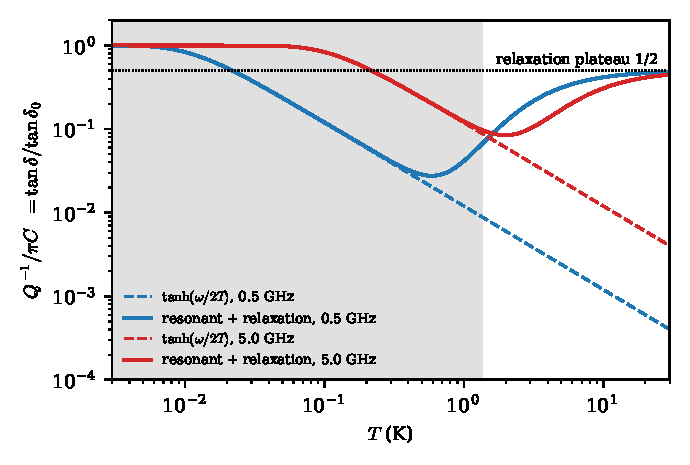
\includegraphics[width=0.82\linewidth]{figures/ch16/limit16_7a.pdf}
\captionof{figure}{Loss of the ensemble in vitreous silica, divided by its value at $T = 0$, against temperature, at \SI{0.5}{GHz} (blue) and \SI{5}{GHz} (red). Dashed: $\tanh(\omega/2T)$. Solid: resonant plus relaxation part, \cref{eq:16.7-relax}, with the one-phonon rate \cref{eq:16.7-tau1} for $\rho_T = \SI{2.2}{g.cm^{-3}}$, $c_{\mathrm{LA}} = 5.8$ and $c_{\mathrm{TA}} = \SI{3.8}{km.s^{-1}}$~\cite[Table~I]{buchenau2020sound}, an assumed $\gamma_{\mathrm{l}} = \SI{1}{eV}$ and $\gamma_{\mathrm{l}}/\gamma_{\mathrm{t}} = 1.6$~\cite{zhou2015generic}, so that $K_{\mathrm{ph}} = \SI{4.63e4}{eV^{-2}}$. Dotted: the relaxation plateau. Gray: the full loss within \SI{10}{\percent} of the tanh law at \SI{5}{GHz}, $T < \SI{1.36}{K}$ (\SI{0.43}{K} at \SI{0.5}{GHz}).}\label{fig:16-limit-tls}
\par}
\smallskip
Above these temperatures the population of slowly relaxing systems lags the field, and the loss rises toward the plateau $\tan\delta_0/2$ instead of falling as $\omega/2T$.
\end{limitbox}

\Cref{lim:16.7a} puts the relaxation correction where the low-temperature estimate puts it: \SI{10}{\percent} of the resonant loss at $T = [0.6\,\omega^2/(\pi^3K_{\mathrm{ph}})]^{1/4}$, which is \SI{1.34}{K} at \SI{5}{GHz} against \SI{1.36}{K} from the full integral. At \SI{10}{mK} the relaxation part at \SI{5}{GHz} is $4\times10^{-9}$ of the resonant one. The value of $\gamma_{\mathrm{l}}$ enters only through $K_{\mathrm{ph}}$, and since the crossover temperature scales as $K_{\mathrm{ph}}^{-1/4}$, a deformation potential twice as large moves it down by a factor $2^{1/2}$. The tunneling model has its own limits at these temperatures: above about \SI{2}{K}, relaxation by several phonons adds to \cref{eq:16.7-tau1}~\cite[Sect.~II]{meissner2021acoustic}. The second correction is saturation. A field strong enough to drive transitions faster than the systems relax equalizes the two populations and removes the resonant loss; for sound the resonant term falls as $[1 + I/I_{\mathrm{c}}]^{-1/2}$ with the intensity $I$, and the critical intensity is $\sim10^{-7}\,\si{W.cm^{-2}}$~\cite[Eq.~(8)]{buchenau2020sound}. This is why the resonator loss falls at high power and why $\tan\delta_0$ is the low-power value. In practice the tunneling parameters, the distributions of $\Delta_{\mathrm{as}}$ and $\lambda_{\mathrm{tun}}$, the deformation potentials and the dipole moments, are computed from ensembles of model glasses, found by searching their energy landscapes for pairs of nearby minima (\cref{app:E.22}). The computed $\bar Pp_{\mathrm{TLS}}^2$ is then checked against the measured $\tan\delta_0$ of the same preparation.

\subsection{Dark-photon absorption on two-level systems}\label{sec:16.7-dp}

A dark photon of mass $m_\phi$ is absorbed at the rate per unit target mass $\mathcal{R} = (\rho_\chi/\rho_T)\zeta^2L(m_\phi)$, with $L = \Imag(-1/\varepsilon)$ the loss function at $\vect{p}_\phi \to 0$ (\cref{eq:10.7-dp}). The momentum $\vect{p}_\phi \approx m_\phi v$ of a dark photon of \SI{25}{\micro eV} is $3\times10^{-8}\,\si{eV}$ for $v = \SI{354}{km.s^{-1}}$, a wavelength of about \SI{40}{m}, so the local dielectric function of the glass is all we need. For a glass with $\varepsilon = \varepsilon_r(1 + \ii\tan\delta)$ the loss function is $\tan\delta/[\varepsilon_r(1 + \tan^2\delta)]$, and with \cref{eq:16.7-tand},
\begin{keyresult}[Dark-photon absorption on two-level systems]
\begin{equation}
  \mathcal{R} = \frac{\rho_\chi}{\rho_T}\,\zeta^2\,\frac{\tan\delta_0}{\varepsilon_r}\,\tanh\frac{m_\phi}{2T}\,\bigl[1 + \mathcal{O}(\tan^2\delta_0)\bigr] .
  \label{eq:16.7-dp}
\end{equation}
The rate per unit mass is independent of $m_\phi$ wherever $m_\phi \gg 2T$, and it is fixed by two measured numbers, the low-power loss tangent and the permittivity.
\end{keyresult}
\noindent The factor $\tanh(m_\phi/2T)$ appears once. It is the population difference of the absorbing systems, and the net rate already subtracts the stimulated emission that the dark-matter field drives from the upper level, just as the dielectric loss does; a second thermal factor from the field would count that subtraction twice. The in-medium suppression $1/\varepsilon_r$ is the factor $1/|\varepsilon|^2$ of \cref{eq:10.7-dp} times the $\varepsilon_r$ in $\varepsilon_2 = \varepsilon_r\tan\delta$: the field inside the glass is screened, and the absorbers respond to the screened field. And the dark-matter field drives each system far below saturation. At the coupling that \cref{we:16-tls-dp} finds for three events per kg-year, the field $\zeta(2\rho_\chi)^{1/2}$ of \cref{sec:11.8} gives a Rabi frequency below $6\times10^{-7}\,\si{s^{-1}}$ for a dipole of \SI{1.1}{D}, against a relaxation rate of $10^6\,\si{s^{-1}}$ for a system with $\Delta_{\mathrm{tl}} = m_\phi$ at \SI{6}{GHz}.

What the two-level systems add is a loss that is flat in frequency, from the lowest masses at which $m_\phi$ exceeds $2T$ up to the energies at which the flat distribution \cref{eq:16.7-P} ceases to hold. The loss tangents that fix the rate are measured near \SI{6}{GHz} (\SI{25}{\micro eV}) and below \SI{100}{mK}, and they depend on how the oxide was made. Thermal SiO$_2$ has $\tan\delta_0 = 3.0$ to $3.3\times10^{-4}$, and oxide deposited from a plasma $2.7$ to $2.9\times10^{-3}$ in lumped-element resonators~\cite[Table~I]{oconnell2008microwave}. A second deposited oxide reached $5\times10^{-3}$~\cite{martinis2005decoherence}. Such films are a few hundred nanometers thick, and no millikelvin value has been measured for bulk fused silica.

\begin{workedexample}{The dark-photon rate on thermal SiO$_2$}\label{we:16-tls-dp}
Take thermal SiO$_2$ with $\tan\delta_0 = 3\times10^{-4}$, an assumed static permittivity $\varepsilon_r = 3.9$, and $\rho_T = \SI{2.2}{g.cm^{-3}}$, at $T = \SI{10}{mK}$ ($T = \SI{0.862}{\micro eV}$). A dark photon of \SI{6}{GHz}, $m_\phi = \SI{24.81}{\micro eV}$, has $m_\phi/2T = 14.4$, so $\tanh(m_\phi/2T) = 1$ to eight digits, and the loss function is $L = 3\times10^{-4}/3.9 = \num{7.69e-5}$. The prefactor is $\rho_\chi/\rho_T = (\SI{0.3}{GeV.cm^{-3}})/(\SI{2.2}{g.cm^{-3}}) = \SI{0.136}{GeV/g}$, which divided by $\hbar$ is $2.07\times10^{23}$ per gram per second. Then
\begin{equation*}
  \mathcal{R} = \num{5.03e29}\,\zeta^2\ \text{per kg-year} ,
\end{equation*}
and three events in one kg-year need $\zeta = \num{2.44e-15}$. The upper end of the measured range, $3.3\times10^{-4}$, raises the rate by 1.10, and the deposited oxide with $5\times10^{-3}$ by 16.7, which lowers $\zeta$ by a factor 0.24. At \SI{100}{mK} the thermal factor drops to 0.894, which is why a loss tangent quoted at that temperature must be divided by 0.894 to give $\tan\delta_0$.

The target mass is the problem. A film of \SI{1}{\micro m} on \SI{100}{cm^2} weighs \SI{22}{mg}, and three events in a year then need $\zeta = \num{5.2e-13}$. Each absorption leaves \SI{24.8}{\micro eV} in one two-level system, which decays by emitting a phonon of that energy. The loss tangent also fixes $\bar Pp_{\mathrm{TLS}}^2 = 3\varepsilon_r\tan\delta_0/\pi$ and nothing else: with $\bar P = \SI{1.2e20}{eV^{-1}.cm^{-3}}$, the value that the polarization-averaged $C = 2.6\times10^{-4}$ implies for $\gamma_{\mathrm{l}} = \SI{1}{eV}$, \cref{eq:16.7-tand} requires $p_{\mathrm{TLS}} = 0.23\,e\,\text{\AA} = \SI{1.1}{D}$.
\end{workedexample}

\begin{limitbox}[Dark-photon absorption on two-level systems][lim:16.7b]
$\mathcal{R} = (\rho_\chi/\rho_T)\zeta^2\tan\delta_0\tanh(m_\phi/2T)/\varepsilon_r$, the loss function $\Imag(-1/\varepsilon) = \varepsilon_2/|\varepsilon|^2$ of \cref{eq:10.7-dp} with the electric loss of the tunneling model~\cite[Eq.~(20)]{muller2019towards}.
\par\smallskip
{\centering
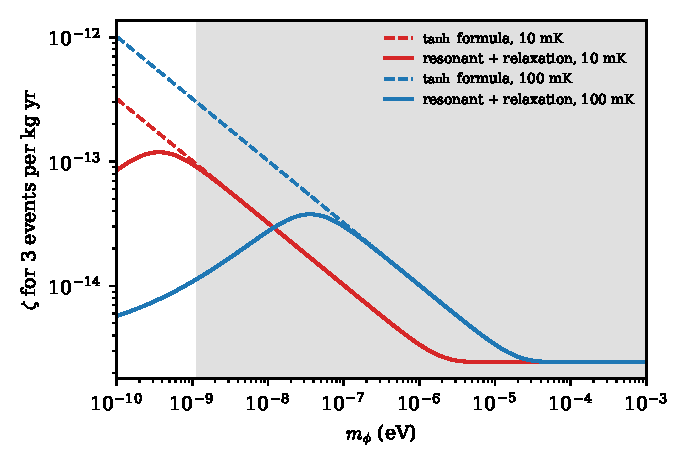
\includegraphics[width=0.82\linewidth]{figures/ch16/limit16_7b.pdf}
\captionof{figure}{Kinetic mixing for three absorptions per kg-year on thermal SiO$_2$ ($\tan\delta_0 = 3\times10^{-4}$, $\varepsilon_r = 3.9$, $\rho_T = \SI{2.2}{g.cm^{-3}}$), against the dark-photon mass, at \SI{10}{mK} (red) and \SI{100}{mK} (blue). Dashed: \cref{eq:16.7-dp}. Solid: $\varepsilon_2/|\varepsilon|^2$ with $\varepsilon_2$ from the resonant plus relaxation loss \cref{eq:16.7-relax}, $K_{\mathrm{ph}}$ as in \cref{fig:16-limit-tls}. Gray: within \SI{10}{\percent} at \SI{10}{mK}, $m_\phi > \SI{1.15}{neV}$ (\SI{0.28}{MHz}); at \SI{100}{mK} the bound moves to \SI{115}{neV}.}\label{fig:16-limit-dp}
\par}
\smallskip
Below these masses the relaxation of systems with splittings near $T$ absorbs more than the resonant systems at $\Delta_{\mathrm{tl}} = m_\phi$, whose population difference vanishes as $m_\phi/2T$.
\end{limitbox}

\noindent The mass of \cref{lim:16.7b} scales as $T^2$: with $\tanh(m_\phi/2T) \approx m_\phi/2T$ and the low-temperature relaxation part $(\pi^3/12)K_{\mathrm{ph}}T^3/m_\phi$, the two are in the ratio $(\pi^3/6)K_{\mathrm{ph}}T^4/m_\phi^2$, which reaches 0.1 at $m_\phi \propto T^2$. Above a millielectronvolt the vibrations of the glass absorb more than its two-level systems (\cref{sec:16.7-ir}).

\subsection{Dark-matter scattering on two-level systems}\label{sec:16.7-scat}

A dark-matter particle that couples to the electron density sees a two-level system through the change of that density between the two configurations. Projected on $|\mathrm{L}\rangle$ and $|\mathrm{R}\rangle$, the density operator at momentum $\vect{q}$ is $\tfrac12(n_{\mathrm{LL}} + n_{\mathrm{RR}}) - \tfrac12f_{\mathrm{TLS}}(\vect{q})\,\sigma_z$, up to terms of relative order $\ee^{-\lambda_{\mathrm{tun}}}$, with the vertex
\begin{equation}
  f_{\mathrm{TLS}}(\vect{q}) = \langle\mathrm{R}|n_e(\vect{q})|\mathrm{R}\rangle - \langle\mathrm{L}|n_e(\vect{q})|\mathrm{L}\rangle .
  \label{eq:16.7-f}
\end{equation}
The first term is the static density and scatters elastically; the second flips the system with the amplitude of \cref{eq:16.7-rot}, $|\langle e|n_e(\vect{q})|g\rangle|^2 = \tfrac14|f_{\mathrm{TLS}}|^2(\Delta_0/\Delta_{\mathrm{tl}})^2$. The structure factor of \cref{eq:2.5-golden} sums this over systems, with the weights $p_0$ and $p_1$ of \cref{sec:2.5} for absorption at $\omega = \Delta_{\mathrm{tl}}$ and emission at $\omega = -\Delta_{\mathrm{tl}}$, and with \cref{eq:16.7-P,eq:16.7-norm} the ensemble gives
\begin{equation}
  S(\vect{q},\omega) = \frac{\pi}{2}\,\bar P\,\bigl\langle|f_{\mathrm{TLS}}(\vect{q})|^2\bigr\rangle\,\frac{1}{1 + \ee^{-\omega/T}} ,
  \label{eq:16.7-S}
\end{equation}
flat in $\omega$ inside the band of the two-level systems and obeying detailed balance, \cref{eq:2.5-db}, as \cref{fig:16-tls}(b) shows. The average runs over the systems and their orientations.

The vertex has two parts. The atoms that tunnel carry their electrons from one well to the other, the core term. And the surrounding glass relaxes elastically around each configuration, which moves all its electrons, the host term. For the host term take the defect as an elastic dipole. In configuration R it exerts on the glass a force dipole that differs from that of L by $-2\gamma_{\mathrm{TLS}}$ along its deformation, since the energy of a force dipole $\mathsf{D}$ in a strain is $-\sum_{\alpha\beta}\mathsf{D}_{\alpha\beta}u_{\alpha\beta}$ and the asymmetry shifts by $2\gamma_{\mathrm{TLS}}u_{\mathrm{d}}$. In an isotropic continuum the static displacement field of a force dipole has longitudinal Fourier component $\vect{q}\cdot\tilde{\vect{u}}(\vect{q}) = -\ii\,\hat{\vect{q}}\cdot\mathsf{D}\cdot\hat{\vect{q}}/\rho_Tc_{\mathrm{LA}}^2$, and since the adiabatic electrons follow the atoms, the electron density changes by $\delta n_e(\vect{q}) = \ii\nd_e\,\vect{q}\cdot\tilde{\vect{u}}$ with $\nd_e$ the density of all electrons. Hence
\begin{equation}
  f_{\mathrm{host}} = \frac{2\nd_e\,\hat{\vect{q}}\cdot\gamma_{\mathrm{TLS}}\cdot\hat{\vect{q}}}{\rho_Tc_{\mathrm{LA}}^2} ,
  \qquad
  \bar P\,\bigl\langle|f_{\mathrm{host}}|^2\bigr\rangle = \frac{4\nd_e^2\,C_{\mathrm{l}}}{\rho_Tc_{\mathrm{LA}}^2} ,
  \label{eq:16.7-host}
\end{equation}
where the orientation average of $(\hat{\vect{q}}\cdot\gamma_{\mathrm{TLS}}\cdot\hat{\vect{q}})^2$ is $\gamma_{\mathrm{l}}^2$, the coupling to longitudinal strain. The deformation potential drops out of the product: the host term of the scattering rate is fixed by the measured tunneling strength $C_{\mathrm{l}}$, not by the loss tangent. The form holds in a window of momentum transfers. The momentum transfer must be static, $q \gg \omega/c_{\mathrm{LA}}$; for $\omega$ near $c_{\mathrm{LA}}q$ the elastic response has a pole, and the process becomes the emission of a real phonon that the two-level system absorbs later, which belongs to the phonon channel of \cref{sec:11.1}. The wavelength must also be long against the defect and the atomic spacing, where continuum elasticity holds. No dielectric factor is added: the adiabatic density already contains the screening of the electrons.

For the core term the simplest model moves one oxygen ion, with its eight electrons, rigidly by $\vect{d}$. With the origin at the midpoint, $f_{\mathrm{core}} = 8(\ee^{\ii\vect{q}\cdot\vect{d}/2} - \ee^{-\ii\vect{q}\cdot\vect{d}/2}) = 16\ii\sin(\vect{q}\cdot\vect{d}/2)$, and its orientation average is $\langle|f_{\mathrm{core}}|^2\rangle = 128[1 - \sin(qd)/qd]$. The core amplitude is imaginary and the static host amplitude is real, so the two add without interference, for every orientation and not only on average; an off-center core would restore a cross term. For a displacement along $\hat{\vect{q}}$ the two are equal near $q_\times = |f_{\mathrm{host}}|/(8d)$, where the host term stops dominating; with the orientation-averaged core, $\langle|f_{\mathrm{core}}|^2\rangle^{1/2} \simeq 4.62\,qd$, the crossing moves up by $\sqrt3$.

With a heavy mediator, $\mathfrak{D}_{ee} = \pi\sigmae/\mu_{\chi e}^2$ and the structure factor \cref{eq:16.7-S} in the isotropic rate \cref{eq:10.1-rateiso}, the minimum velocity is $q/2\mchi$ up to $\omega/q$, negligible for $\omega \lesssim \SI{0.1}{meV}$, and a $q$-independent vertex leaves $\int q\,\dd q\,\eta(q/2\mchi) = 2\mchi^2\langle v\rangle$. The rate is
\begin{equation}
  \frac{\dd\mathcal{R}}{\dd\omega} = \frac{\rho_\chi}{\mchi\rho_T}\,\langle v\rangle\,\sigmae\Bigl(1 + \frac{\mchi}{m_e}\Bigr)^2\,\frac{\bar P\langle|f_{\mathrm{TLS}}|^2\rangle}{4\,(1 + \ee^{-\omega/T})} ,
  \label{eq:16.7-rate}
\end{equation}
per unit energy and target mass, a cross-section $\sigmae(1 + \mchi/m_e)^2|f_{\mathrm{TLS}}|^2(\Delta_0/\Delta_{\mathrm{tl}})^2/4$ per system. The factor $(1 + \mchi/m_e)^2 = \mchi^2/\mu_{\chi e}^2$ converts the reference cross-section on a free electron into the cross-section on a heavy target. For a $q$-dependent core vertex the $q$ integral is done with $\eta$.

Consider amorphous SiO$_2$ at $\mchi = \SI{1}{MeV}$ and $\sigmae = \SI{e-38}{cm^2}$. Thirty electrons per formula unit at \SI{2.2}{g.cm^{-3}} give $\nd_e = \SI{6.62e23}{cm^{-3}}$, and $\rho_Tc_{\mathrm{LA}}^2 = \SI{7.40e10}{Pa} = \SI{4.62e23}{eV.cm^{-3}}$. With the measured longitudinal $C_{\mathrm{l}} = 1.9\times10^{-4}$, \cref{eq:16.7-host} gives $\bar P\langle|f_{\mathrm{host}}|^2\rangle = \SI{7.20e20}{eV^{-1}.cm^{-3}}$, and with the halo of \cref{tab:1-shm}, $\langle v\rangle = \SI{354.1}{km.s^{-1}}$, and $(1 + \mchi/m_e)^2 = 8.74$, the host term is $6.6\times10^{-3}$ per kg, day and meV. The core term needs $\bar P$ itself. For an assumed $\gamma_{\mathrm{l}} = \SI{1}{eV}$, $\bar P = C_{\mathrm{l}}\rho_Tc_{\mathrm{LA}}^2/\gamma_{\mathrm{l}}^2 = \SI{8.8e19}{eV^{-1}.cm^{-3}}$, $|f_{\mathrm{host}}| = 2.86$, and one oxygen moving by \SI{1}{\angstrom} adds $1.6\times10^{-2}$, 2.5 times the host term. The total,
\begin{equation*}
  \frac{\dd\mathcal{R}}{\dd\omega} \approx 2.3\times10^{-2}\ \text{per kg, day and meV} \qquad (\mchi = \SI{1}{MeV},\ \sigmae = \SI{e-38}{cm^2}),
\end{equation*}
is flat over the band of the two-level systems, and over $0 < \omega < \SI{0.1}{meV}$ it amounts to $2.3\times10^{-3}$ events per kg-day. The polarization-averaged $C = 2.6\times10^{-4}$ would raise both terms by 1.37, to $3.1\times10^{-2}$ per kg, day and meV.

This number is an estimate, uncertain by about a factor 3. The heavy-mediator weight $q\,\eta(q/2\mchi)$ has its median at $q = \SI{1.73}{keV}$, where $qd = 0.88$ for $d = \SI{1}{\angstrom}$. The host and core terms cross lower, at $q_\times = \SI{0.71}{keV}$ for a displacement along $\hat{\vect{q}}$ and \SI{1.2}{keV} on orientation average. Most of the rate therefore comes from momentum transfers outside the window of \cref{eq:16.7-host}, near the scale at which the glass stops being a continuum. The core term is a rigid ion, which misses the redistribution of the valence electrons of the moving oxygen, and one geometry stands for many. Both are replaced by the density difference \cref{eq:16.7-f} from two self-consistent calculations of the same glass cell, averaged over an ensemble of systems. Whatever its value, the rate is small because $\bar P$ times the band of energies, about $10^{16}$ systems per cm$^3$, is a small number of targets, and each takes at most \SI{0.1}{meV}. Thin films under a sensor hold far less mass still and matter as absorbers of phonons and as sources of delayed heat (\cref{sec:16.8}), not as targets.

\subsection{Vibrational absorption of glasses}\label{sec:16.7-ir}

In a crystal a dark photon is absorbed on phonons only at the zone-center optical frequencies, where its tiny momentum matches a mode (\cref{sec:11.8}). A glass has no zone center. Every vibrational mode can carry a dipole, and the absorption is spread over the whole vibrational spectrum~\cite{bloch2026dark}. The rate is still $\mathcal{R} = (\rho_\chi/\rho_T)\zeta^2L(m_\phi)$, now with the dielectric function of the vibrations of the glass~\cite[Eq.~(2)]{bloch2026dark}, and the question is what fixes $L$ at the lowest masses.

Take one configuration of the glass in the harmonic approximation, with modes $\nu$ of frequency $\omega_\nu$, eigenvectors $\vect{e}_{I\nu}$ normalized over all $N$ atoms, masses $M_I$ and Born charges $Z^*_I$. Its dielectric function has the rank-one form of \cref{sec:11.8}, with the Hessian of the glass in place of the dynamical matrix,
\begin{equation}
  \varepsilon(\omega) = \varepsilon_\infty + \frac{e^2}{\Vol}\sum_\nu\frac{|p_\nu|^2}{\omega_\nu^2 - \omega^2 - \ii\omega\varGamma_\nu} ,
  \qquad p_\nu = \sum_I\frac{\hat{\boldsymbol{\epsilon}}\cdot Z^*_I\cdot\vect{e}_{I\nu}}{M_I^{1/2}} ,
  \label{eq:16.7-epsglass}
\end{equation}
for a field along $\hat{\boldsymbol{\epsilon}}$ and mode widths $\varGamma_\nu$. For narrow modes the imaginary part is $\varepsilon_2(\omega) = (\pi e^2/2\omega\Vol)\sum_\nu|p_\nu|^2\delta(\omega - \omega_\nu)$. With the vibrational density of states $g(\omega)$ normalized to one, $\sum_\nu\delta(\omega - \omega_\nu) = 3Ng(\omega)$, and with the infrared coupling $C^{\mathrm{IR}}(\omega)$, the mean of $|p_\nu|^2$ over the modes at frequency $\omega$,
\begin{equation}
  \varepsilon_2(\omega) = \frac{3\pi e^2\nd_{\mathrm{at}}}{2\omega}\,g(\omega)\,C^{\mathrm{IR}}(\omega) .
  \label{eq:16.7-eps2}
\end{equation}
The absorption coefficient $\alpha_{\mathrm{abs}} = \omega\varepsilon_2/n_r$, with $n_r = \varepsilon_r^{1/2}$ the refractive index, is then a product of the density of states and a coupling, the form in which infrared spectroscopy of glasses is analyzed~\cite[Eq.~(2) and text before Eq.~(1)]{taraskin2006universal}.

Below the Ioffe--Regel frequency $\omega_{\mathrm{IoR}}$, the frequency at which the mean free path of a vibration falls to one wavelength, the modes are still sound waves, scattered weakly by the disorder. For a plane wave of branch $\nu$ with sound speed $c_\nu$, wavevector $\vect{k}$ and polarization $\hat{\vect{e}}_\nu$, every atom moves with the same velocity, $\vect{e}_{I\nu} = \hat{\vect{e}}_\nu\ee^{\ii\vect{k}\cdot\vect{x}_I}(M_I/N\bar M)^{1/2}$ with $\bar M$ the mean atomic mass. The masses cancel in $p_\nu$, which becomes a Fourier component of the field of Born charges, and averaged over the modes at fixed $\omega = c_\nu k$,
\begin{equation}
  C^{\mathrm{IR}}(\omega) = \frac{1}{\bar M}\sum_\nu\hat w_\nu\,S^Z_\nu(\omega/c_\nu) ,
  \qquad S^Z_\nu(k) = \frac1N\Bigl\langle\Bigl|\sum_I\hat{\boldsymbol{\epsilon}}\cdot Z^*_I\cdot\hat{\vect{e}}_\nu\,\ee^{\ii\vect{k}\cdot\vect{x}_I}\Bigr|^2\Bigr\rangle ,
  \label{eq:16.7-CIR}
\end{equation}
with $\hat w_\nu = c_\nu^{-3}/\sum_{\nu'}c_{\nu'}^{-3}$ the fraction of modes at fixed $\omega$ in branch $\nu$, as in \cref{eq:E.19-CIR}. The behavior of $S^Z_\nu$ at small $k$ decides the low-frequency absorption. A crystal has $S^Z_\nu(k) = 0$ for acoustic modes as $k \to 0$, since the Born charges of a cell add to zero. In a glass the charges fluctuate from site to site. If they obey only global neutrality, uncorrelated fluctuations leave $S^Z_\nu(0^+)$ equal to the mean square fluctuation of the projected charge, a constant. If instead they are neutral within every local unit, as within the SiO$_4$ tetrahedra of silica, the sum is that of dipoles and $S^Z_\nu \propto k^2$. Expanding to second order,
\begin{equation}
  C^{\mathrm{IR}}(\omega) = A^{\mathrm{IR}} + B^{\mathrm{IR}}\omega^2 , \qquad
  A^{\mathrm{IR}} = \frac{1}{\bar M}\sum_\nu\hat w_\nu S^Z_\nu(0^+) , \quad
  B^{\mathrm{IR}} = \frac{1}{\bar M}\sum_\nu\frac{\hat w_\nu S^{Z\prime\prime}_\nu(0)}{2c_\nu^2} ,
  \label{eq:16.7-AB}
\end{equation}
the law Taraskin, Simdyankin, Elliott, Neilson and Lo found in terahertz spectra of glasses~\cite[Eq.~(1)]{taraskin2006universal}. Their fit to vitreous silica at room temperature writes $\alpha_{\mathrm{abs}} = (A^{\mathrm{IR}} + B^{\mathrm{IR}}\tilde\omega^2)g(\tilde\omega)$ in spectroscopic units, with $\alpha_{\mathrm{abs}}$ and the wavenumber $\tilde\omega = \omega/2\pi c$ in cm$^{-1}$ and $g$ normalized per cm$^{-1}$. It gives $A^{\mathrm{IR}} = \SI{4000}{cm^{-2}}$ and $B^{\mathrm{IR}} = 0.3$, dimensionless, with the Debye density of states of a \SI{330}{K} Debye temperature~\cite[Fig.~1]{taraskin2006universal}. Harmonic absorption is net absorption and does not depend on temperature, but a room-temperature spectrum also contains anharmonic and relaxational absorption whose size at millikelvin temperatures has not been separated; there the fit is a model value.

\begin{limitbox}[Glass absorption below the Ioffe--Regel frequency][lim:16.7d]
$\alpha_{\mathrm{abs}}(\omega) = (A^{\mathrm{IR}} + B^{\mathrm{IR}}\tilde\omega^2)\,g(\tilde\omega)$ for $\omega < \omega_{\mathrm{IoR}}$~\cite[Eq.~(1)]{taraskin2006universal}, inserted in the rate $(\rho_\chi/\rho_T)\zeta^2\Imag(-1/\varepsilon)$~\cite[Eq.~(2)]{bloch2026dark}.
\par\smallskip
{\centering
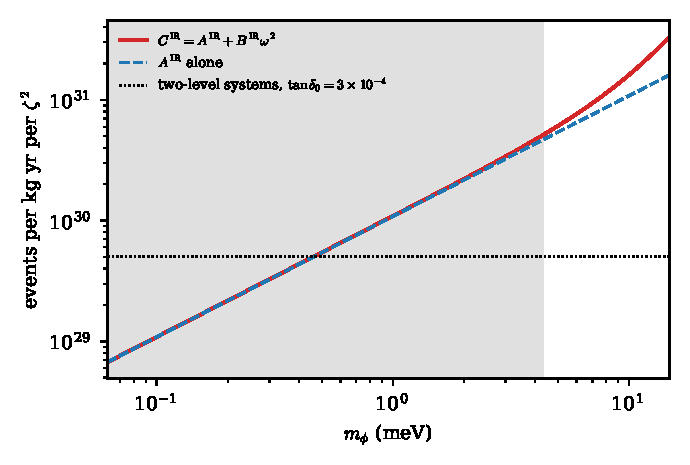
\includegraphics[width=0.82\linewidth]{figures/ch16/limit16_7d.pdf}
\captionof{figure}{Dark-photon absorptions per kg-year per $\zeta^2$ in vitreous silica against the mass, from \cref{eq:16.7-eps2} with $C^{\mathrm{IR}} = A^{\mathrm{IR}} + B^{\mathrm{IR}}\omega^2$ (red) and with the constant term alone (blue, dashed). Inputs: the terahertz fit $A^{\mathrm{IR}} = \SI{4000}{cm^{-2}}$, $B^{\mathrm{IR}} = 0.3$ of Taraskin et al., a Debye density of states with $\Theta_{\mathrm{D}} = \SI{330}{K}$, $\varepsilon_r = 3.9$ and $\rho_T = \SI{2.2}{g.cm^{-3}}$. Dotted: two-level absorption, \cref{eq:16.7-dp}, for thermal SiO$_2$ at saturation. Gray: below the Ioffe--Regel frequency of silica, $\omega/2\pi c \approx \SI{35}{cm^{-1}}$ (\SI{4.3}{meV}), where the $B$ term is at most \SI{9}{\percent} of the $A$ term.}\label{fig:16-limit-ir}
\par}
\smallskip
Above $\omega_{\mathrm{IoR}}$ the modes are no longer plane waves, $S^Z_\nu$ at one wavevector no longer describes them, and the coupling departs from $A^{\mathrm{IR}} + B^{\mathrm{IR}}\omega^2$ in a way that depends on the glass.
\end{limitbox}

\Cref{lim:16.7d} shows how the two channels of a glass divide the masses. With $\varepsilon_2 = n_r\alpha_{\mathrm{abs}}/(2\pi\tilde\omega)$, the vibrational absorption grows as $\omega$ times $C^{\mathrm{IR}}$. At \SI{1.24}{meV} ($\tilde\omega = \SI{10}{cm^{-1}}$) it gives $\alpha_{\mathrm{abs}} = \SI{0.10}{cm^{-1}}$, $\varepsilon_2 = \num{3.1e-3}$ and $1.4\times10^{30}\zeta^2$ absorptions per kg-year. It equals the two-level absorption of thermal SiO$_2$ at \SI{0.46}{meV}, and that of the deposited oxide with $\tan\delta_0 = 5\times10^{-3}$ at \SI{6.4}{meV}, an extrapolation above $\omega_{\mathrm{IoR}}$. The constant term carries the low-frequency absorption of silica entirely: the curvature term reaches the constant only at $\tilde\omega = (A^{\mathrm{IR}}/B^{\mathrm{IR}})^{1/2} = \SI{115}{cm^{-1}}$, three times above $\omega_{\mathrm{IoR}}$. That constant is the incoherent sum of random charges, and a model of the glass that makes every tetrahedron neutral by construction misses it (\cref{app:E.19}). Bloch, Knapen, Li, Madden and Marocco propose amorphous membranes for masses of 50 to \SI{200}{meV}, above $\omega_{\mathrm{IoR}}$, where the mean free path of a mode is shorter than its wavelength and the absorption follows from the measured or computed $\varepsilon(\omega)$ of \cref{eq:16.7-epsglass}~\cite{bloch2026dark}. The same random couplings give a broadband absorption in a crystal with isotope disorder, which \cref{sec:11.6} treats.

\subsection{Random media and the Born limit}\label{sec:16.7-random}

A dark-matter particle of \SI{20}{eV} moving at $v = 10^{-3}$ has a de Broglie wavelength $2\pi/\mchi v$ of about \SI{60}{\micro m}. A momentum transfer $\sim\mchi v$ cannot resolve atoms, and the particle scatters off the smoothed density $\nd(\vect{r})$ of nucleons of a whole body. Liu, Matsumoto, Sheng and Xing pointed out that a random two-phase material scatters such particles far more strongly than a homogeneous one~\cite{liu2025coherence}. In the first Born approximation for the body, the amplitudes of all nucleons add with their phases, and for a spin-independent interaction
\begin{equation}
  \frac{\dd\sigma_{\mathrm{tot}}}{\dd\Omega_q} = \frac{\dd\sigma_{\chi N}}{\dd\Omega_q}\,\Bigl|\int\dd^3r\,\ee^{\ii\vect{q}\cdot\vect{r}}\,\nd(\vect{r})\Bigr|^2 ,
  \label{eq:16.7-born}
\end{equation}
the coherent sum of \cref{sec:2.2} with the nucleus replaced by the body~\cite[Eq.~(2)]{liu2025coherence}. Write $\nd = \nd_0 + \delta\nd$ with $\nd_0$ the mean nucleon density, and average over the random structure. The cross term vanishes, and the two remaining terms are the homogeneous body, $\nd_0^2|\int_{\Vol}\dd^3r\,\ee^{\ii\vect{q}\cdot\vect{r}}|^2$, which falls as $(qR)^{-4}$ for a sphere of radius $R$ once $qR \gg 1$, and the fluctuations, $\int\dd^3r_1\dd^3r_2\,\ee^{\ii\vect{q}\cdot(\vect{r}_2 - \vect{r}_1)}\langle\delta\nd(\vect{r}_1)\delta\nd(\vect{r}_2)\rangle$. For a correlation that decays as $\langle\delta\nd(\vect{r}_1)\delta\nd(\vect{r}_2)\rangle = \delta\nd^2\ee^{-|\vect{r}_2 - \vect{r}_1|/\xi_{\mathrm{c}}}$ over a correlation length $\xi_{\mathrm{c}}$, the transform $\int\dd^3r\,\ee^{\ii\vect{q}\cdot\vect{r}}\ee^{-r/\xi_{\mathrm{c}}} = 8\pi\xi_{\mathrm{c}}^3/(1 + q^2\xi_{\mathrm{c}}^2)^2$ times the volume $\Vol = 4\pi R^3/3$ gives, per squared number of nucleons $\nd_0^2\Vol^2$,
\begin{equation}
  |F_{\mathrm{fluc}}(q)|^2 = \frac{\delta\nd^2}{\nd_0^2}\,\frac{6\,\xi_{\mathrm{c}}^3}{R^3(1 + q^2\xi_{\mathrm{c}}^2)^2} ,
  \label{eq:16.7-Ffluc}
\end{equation}
for $R \gg \xi_{\mathrm{c}}$, the result of Ref.~\cite[Eqs.~(9)--(12)]{liu2025coherence}. The body acts as a collection of incoherent clusters of size $\xi_{\mathrm{c}}$, each scattering coherently. At $qR \gg 1$ and $q\xi_{\mathrm{c}} \gg 1$ the sphere-averaged homogeneous term is $9/[2(qR)^4]$, and the ratio of the two is $(4/3)(R/\xi_{\mathrm{c}})(\delta\nd/\nd_0)^2$. For the Ti--6Al--4V alloy of the test masses of the MICROSCOPE satellite test of the equivalence principle, the authors infer $\nd_0 = \SI{2.69e24}{cm^{-3}}$ and $\delta\nd = \SI{7.29e22}{cm^{-3}}$ from the phase fractions of its microstructure~\cite[Eq.~(14)]{liu2025coherence}. Then $(\delta\nd/\nd_0)^2 = 7\times10^{-4}$, and for that value the homogeneous term the authors drop is the larger one below a few hundred eV on an equal-mass sphere.

A large coherent cross-section, however, means a strong interaction with the medium, and the Born approximation for a whole body is not the Born approximation for one nucleus. At wavelengths long against the spacing of nuclei, the medium acts on the particle as an optical potential. It is the sum of the pseudopotentials $2\pi b_{\chi N}/\mu_{\chi N}$ of the nucleons, with $b_{\chi N}$ the scattering length, $\sigma_{\chi N} = 4\pi b_{\chi N}^2$, and $\mu_{\chi N} \approx \mchi$ for a light particle:
\begin{equation}
  V_{\mathrm{opt}} = \frac{2\pi b_{\chi N}\nd_0}{\mu_{\chi N}} .
  \label{eq:16.7-Vopt}
\end{equation}
The plane wave inside the body is undistorted only if this potential is small against the kinetic energy, $|V_{\mathrm{opt}}| \ll E_{\mathrm{kin}} = \mchi v^2/2$. Squaring $|b_{\chi N}| \ll \mchi^2v^2/4\pi\nd_0$ gives the condition on the cross-section,
\begin{equation}
  \sigma_{\chi N} \ll \sigma_{\mathrm{crit}} = \frac{\mchi^4v^4}{4\pi\nd_0^2} ,
  \qquad \frac{|V_{\mathrm{opt}}|}{E_{\mathrm{kin}}} = \Bigl(\frac{\sigma_{\chi N}}{\sigma_{\mathrm{crit}}}\Bigr)^{1/2} .
  \label{eq:16.7-scrit}
\end{equation}
Since $\sigma_{\mathrm{crit}} \propto v^4$, the condition must hold over the velocities that dominate the observable, not at one speed. The homogeneous term of \cref{eq:16.7-born} contains the scattering of the wave by the surface of the body. For a planar face its first-order form can be compared with the exact reflection off a potential step, which shows where the first-order treatment of the medium breaks down. For a wave whose kinetic energy of motion normal to the face is $E_n$, the wavenumber inside is $k' = k(1 - V_{\mathrm{opt}}/E_n)^{1/2}$ and the reflectance is $R_{\mathrm{refl}} = |(k - k')/(k + k')|^2$, total for $V_{\mathrm{opt}} > E_n$. Expanding $k'$ to first order in $V_{\mathrm{opt}}$ gives the Born value $(V_{\mathrm{opt}}/4E_n)^2$, the square of the first-order amplitude of the step.

\begin{limitbox}[Random media and the Born limit][lim:16.7c]
First Born approximation for a whole body, $\dd\sigma_{\mathrm{tot}}/\dd\Omega_q = (\dd\sigma_{\chi N}/\dd\Omega_q)|\int\dd^3r\,\ee^{\ii\vect{q}\cdot\vect{r}}\nd(\vect{r})|^2$, with the fluctuation form factor \cref{eq:16.7-Ffluc}~\cite[Eqs.~(2), (9)--(12), (14)]{liu2025coherence}.
\par\smallskip
{\centering
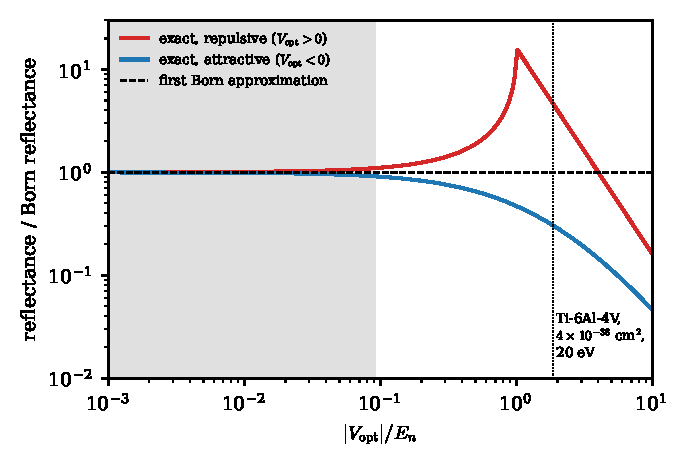
\includegraphics[width=0.82\linewidth]{figures/ch16/limit16_7c.pdf}
\captionof{figure}{Exact reflectance of a planar face of a homogeneous medium with optical potential \cref{eq:16.7-Vopt}, divided by its first Born approximation $(V_{\mathrm{opt}}/4E_n)^2$, against $|V_{\mathrm{opt}}|/E_n$, for a repulsive (red) and an attractive (blue) medium. $E_n$ is the kinetic energy of the motion normal to the face. Gray: the ratio within \SI{10}{\percent} of one, $|V_{\mathrm{opt}}|/E_n < 0.092$. Dotted: $V_{\mathrm{opt}}/E_{\mathrm{kin}} = 1.86$, the value at $\sigma_{\chi N} = \SI{4e-38}{cm^2}$, $\mchi = \SI{20}{eV}$, $v = 10^{-3}$ in Ti--6Al--4V ($\nd_0 = \SI{2.69e24}{cm^{-3}}$).}\label{fig:16-limit-born}
\par}
\smallskip
Beyond $|V_{\mathrm{opt}}| \approx E_n$ a repulsive body reflects every particle that reaches it, and the force on it scales with the optical potential of each material, not with the square of its density fluctuations.
\end{limitbox}

\noindent The leading correction is linear: the ratio of \cref{lim:16.7c} is $1 + V_{\mathrm{opt}}/E_n$ for small $V_{\mathrm{opt}}/E_n$, \SI{1}{\percent} at $V_{\mathrm{opt}}/E_n = 0.01$, of opposite sign for the two signs of the potential. Below $\sigma_{\mathrm{crit}}$ the uniform part of the medium only shifts the wavenumber inside, $k \to k'$, a phase that drops out of the fluctuation term once the wave is distorted by it, and the fluctuation cross-section keeps corrections of relative order $V_{\mathrm{opt}}/E_{\mathrm{kin}}$. In Ti--6Al--4V at $\mchi = \SI{20}{eV}$, \cref{eq:16.7-scrit} gives $\sigma_{\mathrm{crit}} = \SI{1.16e-38}{cm^2}$ at $v = 10^{-3}$, \SI{2.41e-38}{cm^2} at $v = \num{1.2e-3}$ and \SI{5.7e-37}{cm^2} at the largest laboratory speed $v_{\mathrm{max}} = \num{2.650e-3}$. Liu et al.\ quote a reach of $\sigma_{\chi N} \approx \SI{4e-38}{cm^2}$ near \SI{20}{eV} from the MICROSCOPE bound on differential acceleration~\cite[Sect.~IV]{liu2025coherence}, where $|V_{\mathrm{opt}}|/E_{\mathrm{kin}} = 1.86$ at $v = 10^{-3}$ and 1.29 at $v = \num{1.2e-3}$, before the projection on the normal of a face lowers $E_n$ further. At that cross-section the first-order treatment of the medium does not apply to the speeds near the peak of the distribution. Whether the true force on the test masses is larger or smaller than the Born estimate depends on the sign of $b_{\chi N}$, on reflection at the faces and on the composition difference of the two masses. Until the force is computed by transfer matrices over the faces and the velocity distribution, a bound from this channel is a conjecture.

\subsection{Open problems for glass targets}\label{sec:16.7-open}

For a given film the parameters of the standard tunneling model are known only in combination: the loss tangent fixes $\bar Pp_{\mathrm{TLS}}^2$, the acoustic loss $\bar P\gamma_{\mathrm{l}}^2$ and $\bar P\gamma_{\mathrm{t}}^2$, and neither fixes $\bar P$; the core term, the relaxation corrections and the kinetics of \cref{sec:16.8} need all three. For the films of real detectors (amorphous Al$_2$O$_3$ in junctions, SiO$_2$ and SiN$_x$ under sensors, amorphous WSi) these have not been measured on the same sample. Beyond the values, the model itself is an assumption: that $\Delta_{\mathrm{as}}$ and $\lambda_{\mathrm{tun}}$ are independent and flat, at every energy from the lowest masses to the top of the band, and that the systems do not interact. Its successes, the linear specific heat and the logarithmic shift of the sound velocity, test averages, not the distributions, and the ratio $\gamma_{\mathrm{l}}/\gamma_{\mathrm{t}}$, between 1.44 and 1.84 in 18 glasses, is nearly universal without the model giving a reason~\cite{zhou2015generic}. One film measured three ways would settle the first question: the dielectric loss, the acoustic loss, and the strain and field dependence of single systems resolved in a resonator, which give $\gamma_{\mathrm{TLS}}$ and $p_{\mathrm{TLS}}$ directly~\cite{muller2019towards}. The second needs the distributions computed for a model glass of stated preparation.
